\documentclass{standalone}
\usepackage{tikz}

\begin{document}
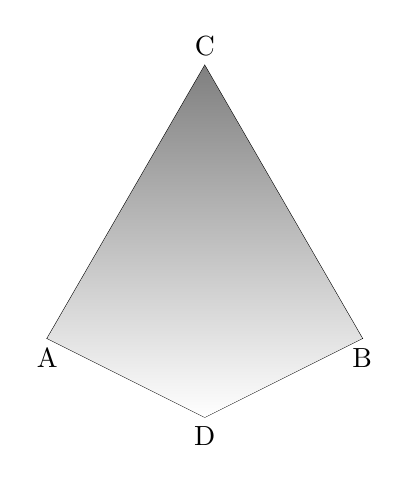
\begin{tikzpicture}[scale=2]
    % Define the vertices of the triangle
    \coordinate (A) at (0, 0);
    \coordinate (B) at (2, 0);
    \coordinate (C) at (1, 1.732);

    % Draw the triangle
    \draw (A) -- (B) -- (C) -- cycle;

    % Define the additional vertex
    \coordinate (D) at (1, -0.5);

    % Connect the additional vertex to each vertex of the triangle
    \draw (D) -- (A);
    \draw (D) -- (B);
    \draw (D) -- (C);

    % Label the vertices
    \node at (A) [below] {A};
    \node at (B) [below] {B};
    \node at (C) [above] {C};
    \node at (D) [below] {D};

    % Add some shading to make it look more like a curve
    \shade[gray!50] (A) -- (D) -- (B) -- cycle;
    \shade[gray!50] (B) -- (D) -- (C) -- cycle;
    \shade[gray!50] (C) -- (D) -- (A) -- cycle;
\end{tikzpicture}
\end{document}